\documentclass[usenames,svgnames,14pt]{beamer}
\usepackage[english]{babel}
\usepackage{
  fontspec,
  fontawesome,
  xcolor,
  mathabx,
  listings,
  lstautogobble,
  listofitems,
  TeXnicalities,
  comment
}

\setsansfont{Yanone Kaffeesatz}[
    UprightFont     = *-Regular ,
    BoldFont        = *-Bold ,
    BoldItalicFont  = *-Bold ,
    BoldSlantedFont = *-Bold ,
    ItalicFont      = *-Light ,
    SlantedFont     = *-Light ,
    SmallCapsFont   = *-Thin
]
\graphicspath{{../Figures/}}
\usetheme[style=green]{Z02}

\usetikzlibrary{
    positioning,
    shapes,
    bbox
}
%Colors for listings
\colorlet{background-color}{gray!20}
\colorlet{basic-color}{black}
\colorlet{keywords-color}{Goldenrod}
\colorlet{comment-color}{red!95!black}
\colorlet{strings-color}{ForestGreen}
\colorlet{builtins-color}{MediumBlue!90!black}
\colorlet{functions-color}{NavyBlue}
\colorlet{variables-color}{DarkOrange}
\colorlet{environment-color}{Gray}
\colorlet{external-color}{SteelBlue}

% https://tex.stackexchange.com/a/34000
\makeatletter
\lst@Key{countblanklines}{true}[t]%
    {\lstKV@SetIf{#1}\lst@ifcountblanklines}

\lst@AddToHook{OnEmptyLine}{%
    \lst@ifnumberblanklines\else%
       \lst@ifcountblanklines\else%
         \advance\c@lstnumber-\@ne\relax%
       \fi%
    \fi}
\makeatother

%listings set
\lstdefinestyle{MyBash}{
backgroundcolor=\color{background-color}, % choose the background color; you must add \usepackage{color} or \usepackage{xcolor}
breakatwhitespace=false,            % sets if automatic breaks should only happen at whitespace
breaklines=true,                    % sets automatic line breaking
captionpos=b,                       % sets the caption-position to bottom
deletekeywords={...},               % if you want to delete keywords from the given language
escapeinside={@|}{|@},              % if you want to add LaTeX within your code
extendedchars=true,                 % lets you use non-ASCII characters; for 8-bits encodings only,
                                    % does not work with UTF-8
frame=single,                       % adds a frame around the code
framerule=0pt,                      % Width of the frame rule
framesep=3pt,                       % separation around text
linewidth=\textwidth,               % defines the base line width for listings
xleftmargin=6mm,                    % Margin left
xrightmargin=6mm,                   % Margin right
numbers=left,                       % where to put the line-numbers; possible values are (none, left, right)
numberblanklines=false,             % suppress numbers on empty lines
countblanklines=false,              % NOT standard! Avoid counting empty lines: https://tex.stackexchange.com/a/34000
numbersep=8pt,                      % how far the line-numbers are from the code
numberstyle=\tiny\color{black},     % the style that is used for the line-numbers
rulecolor=\color{black},            % if not set, the frame-color may be changed on line-breaks within not-black text
                                    % (e.g. comments (green here))
showspaces=false,                   % show spaces everywhere adding particular underscores; it overrides 'showstringspaces'
showstringspaces=false,             % underline spaces within strings only
showtabs=false,                     % show tabs within strings adding particular underscores
stepnumber=1,                       % the step between two line-numbers. If it's 1, each line will be numbered
tabsize=2,                          % sets default tabsize to 2 spaces
title=\lstname,                     % show the filename of files included with \lstinputlisting; also try caption instead of title
%
%Base style for this presentation 
keepspaces=true,                    % keeps spaces in text, useful for keeping indentation of code
                                    % (possibly needs columns=flexible)
language=bash,
basicstyle=\ttfamily\scriptsize\color{basic-color},
keywordstyle=\color{keywords-color},
stringstyle=\color{strings-color},
commentstyle=\color{comment-color},
morestring=[b][\color{strings-color}]{"},
morestring=[d][\color{strings-color}]{'},
moredelim=[is][\color{basic-color}]{|+}{+|}, % I will use this for terminal output
literate={`}{\textasciigrave}1, % https://tex.stackexchange.com/a/466224/128737
literate={~}{{\textasciitilde}}1,
% literate=% literate={<replace>}{<replacement text>}{<width>}
%   {\#define}{{{\color{CarnationPink}\#define}}}{6}
%   {\#include}{{{\color{CarnationPink}\#include}}}{7},
alsoletter=0123456789![]/\{\}.:+, % This to mark the symbols in keyword/emph[5] to be highlighted (otherkeywords does not work i.e. it highlights also in comments!) -> manual at page 45
morekeywords={if, then, else, elif, fi, case, esac, for, select, while, until, do, done, in, function, time, [[, ]], \{, \}, !, coproc}, %https://askubuntu.com/a/513712
emph=[1]{},
emphstyle=[1]{\color{functions-color}}, %Functions
emph=[2]{},
emphstyle=[2]{\color{variables-color}}, %Variables
emph=[4]{PATH, SHELL, IFS, BASH_ALIASES, BASH_REMATCH, PS3, REPLY, HOME, LANGUAGE, EDITOR, PIPESTATUS, PWD, FUNCNEST,
         DIRSTACK, PWD, OLDPWD, SHELLOPTS, BASHOPTS, TIMEFORMAT, COMP_CWORD, COMP_LINE, COMP_POINT, COMP_TYPE, COMP_KEY,
         COMP_WORDBREAKS, COMP_WORDS, COMPREPLY, INPUTRC},
emphstyle=[4]{\color{environment-color}}, %Environment variables
emph=[5]{alias, bg, bind, break, builtin, cd, command, compgen, complete, continue, declare, dirs, disown, echo, enable, eval,
         exec, exit, export, false, fc, fg, getopts, hash, help, history, jobs, kill, let, local, logout, popd, printf, pushd, pwd,
         read, readonly, return, set, shift, shopt, source, suspend, test, times, trap, true, type, typeset, ulimit, umask,
         % case, if, until, while  % <--- these built-in are keywords and I leave them highlighted as such
         unalias, unset, wait, :, ., [, ]},
emphstyle=[5]{\color{builtins-color}}, %Shell built-in
emph=[6]{man, apropos, ls, rm, g++, chmod, cp, awk, sed, cut, perl, args, date, grep, sleep, tput, seq, cat, wc, sort, uniq, tail,
         head, sdiff, tar, mktemp, mkdir, ps, emacs, systemd, timeout, parallel, xargs, gnuplot, pdflatex, vi, ping, bash,
         egrep, shuf, stat, find, fgrep, bc, tr, paste, expr, diff, touch},
emphstyle=[6]{\color{external-color}}, %(External) commands
emph=[7]{},
emphstyle=[7]{\color{variables-color}}, %Class for local variables (usually with bad names)
emph=[8]{},
emphstyle=[8]{\color{builtins-color}}, %Class for local commands (usually with bad names)
%
%Additional customizations
belowskip=-7mm,
aboveskip=3pt,
autogobble=true, % lstautogobble needed!
}

\lstnewenvironment{Bash}[1][] %I will rarely use this because putting a $ in it as prompt breaks down TeXclipse highlight syntax!
    {\lstset{style=MyBash, #1}}
    {}

\def\bash{\lstinline[style=MyBash, basicstyle=\ttfamily\color{black}]}


%===============================================================%
\title{Let's Git together}
\date{XX August 2022}
\author{Alessandro Sciarra}
\institute{Z02~--~Software Development Center}
\titlegraphic{
\includegraphics[width=20mm]{LogoCRC}}
\titlepagelogo{
\includegraphics[width=20mm]{LogoGoethe}}
%===============================================================%

\AtBeginSection[] % <- Empty optional argument, do nothing for \section*
{
    \begin{frame}[plain, noframenumbering]{}
         \sectionpage
    \end{frame}
}

\tikzset{
    space/.style={%
        thick, draw=#1, fill=#1!10, text=#1, rounded corners=1mm, font=\small, text width=14mm, align=center, minimum height=12mm
    }
}
\newcommand{\ttc}[2]{\texttt{\textcolor{#1}{#2}}}
\setlength{\leftmarginii}{0.5cm}
\newcommand{\then}{\raisebox{2pt}{$\;\drsh\;$}}

% Taken from
\makeatletter
\patchcmd{\beamer@sectionintoc}{\vskip1.5em}{\vskip0.5em}{}{}
\makeatother

\begin{document}

%===============================================================%
\begin{frame}[plain,noframenumbering]
    \titlepage
\end{frame}
%~~~~~~~~~~~~~~~~~~~~~~~~~~~~~~~~~~~~~~~~~~~~%
\begin{frame}{Outline of the talk}
    \tableofcontents[subsectionstyle=hide]
\end{frame}
%===============================================================%

%===============================================================%
\section{A short recap from last time}
%~~~~~~~~~~~~~~~~~~~~~~~~~~~~~~~~~~~~~~~~~~~~%
\begin{frame}{By now, this is how your workflow looks like}
    \begin{center}
        \begin{tikzpicture}[node distance=3mm, bezier bounding box] % \usetikzlibrary{bbox}
            \coordinate (N0) at (0,0);
            \foreach \n/\c [count=\i from 0, count=\ip from 1] in {Work/PS, git status git diff/PP, git add/PB, git commit/PT}{
                \begin{scope}[scope on=<1->]
                    \node[space=\c, below = of N\i, xshift=25mm] (N\ip) {\n};
                    \ifnum\i>0%
                    \path[thick, to] (N\i.east) edge[out=0, in=90] (N\ip.north);
                    \fi
                \end{scope}
            }
            \path[visible on=<1->, thick, dotted, to] (N4.west) edge[out=180, in=180, looseness=1.6] (N2.west);
            \path[visible on=<1->, thick, to] (N4.south) edge[out=270, in=180, looseness=1.3] (N1.west);
        \end{tikzpicture}
    \end{center}
\end{frame}
%~~~~~~~~~~~~~~~~~~~~~~~~~~~~~~~~~~~~~~~~~~~~%
\newcommand{\GitCommand}[6][midway]{%
    \draw[#2] ($(N#3.south)!#5!(E#3)$) -- node[#1, fill=BGLIGHT, font=\ttfamily\scriptsize] {#6} ($(N#4.south)!#5!(E#4)$);
}
\begin{frame}{Our mental picture, so far}{On your local machine}
    \vspace{-0.1\textheight}
    \begin{center}
        \begin{tikzpicture}[node distance=25mm]
            \begin{scope}[scope on=<1->]
                \coordinate (N0) at (0,0);
                \foreach \n/\c [count=\i from 0, count=\ip from 1] in {Workspace/PS, Staging area/PP, Local repository/PB}{
                    \node[space=\c, right = of N\i] (N\ip) {\n};
                    \draw[very thin] (N\ip) -- coordinate[pos=1] (E\ip) ++(0,-5);
                }
            \end{scope}
            \begin{scope}[scope on=<1->]
                \node[text=PQ, font=\ttfamily\scriptsize] at ($(N1)!0.5!(N2)$) {git status};
                \node[text=PQ, font=\ttfamily\scriptsize] at ($(N3.north)+(0,0.3)$) {git log};
                \node[text=PQ, font=\ttfamily\scriptsize] at ($(N3.north)+(0,0.7)$) {git show};
                \GitCommand{fromto,PQ}{1}{2}{0.10}{git diff}
                \GitCommand{fromto,PQ}{2}{3}{0.25}{git diff --staged}
                \GitCommand{to}{1}{2}{0.65}{git add}
                \GitCommand{from}{1}{2}{0.80}{git restore --staged}
                \GitCommand{to}{2}{3}{0.95}{git commit}
                \path[to, PQ] ($($(N3.south)!0.45!(E3)$)!0.65!($(N2.south)!0.45!(E2)$)$) edge[out=180, in=0] ($(N2.south)!0.35!(E2)$);
                \GitCommand[pos=0.8]{fromto,PQ}{1}{3}{0.45}{git diff HEAD}
                \node[text=PT] at ($($(N1.south)!0.47!(E1)$)!0.8!($(N3.south)!0.51!(E3)$)$) {\Remark{only tracked files}};
            \end{scope}
        \end{tikzpicture}
        \par\medskip
        {\small Commands marked in \PQ{dark red} do not change anything in the repository!}
        \FrameRemark{Git introduced \texttt{git-restore} in v2.23 but this stayed buggy for a while. Use it from v2.27 on, otherwhise use \texttt{git-reset}.}
    \end{center}
\end{frame}
%~~~~~~~~~~~~~~~~~~~~~~~~~~~~~~~~~~~~~~~~~~~~%
\begin{frame}{The complete correct abstract mental setup}
    \begin{tikzpicture}[node distance=5mm]
        \coordinate (N0) at (0,0);
        \foreach \n/\c [count=\i from 0, count=\ip from 1] in {Stashing area/PQ, Workspace/PS, Staging area/PP, Local repository/PB, Remote repository/PT}{
            \node[space=\c, right = of N\i] (N\ip) {\n};
            \draw[very thin] (N\ip) -- coordinate[pos=1] (E\ip) ++(0,-5);
        }
        \path coordinate (DNE) at ($(N4.north east)!0.5!(N5.north west)+(0,1)$)
              coordinate (DSE) at ($(DNE)-(0,7.1)$)
              coordinate (DNW) at ($(N1.north east)!0.5!(N2.north west)+(0,1)$)
              coordinate (DSW) at ($(DNW)-(0,7.1)$);
        \draw[thin, dashed] (DNE) -- (DSE);
        \draw ($(N1.north west)-(0.1,0)$) -- ++(0,0.2) -| ($(N4.north east)+(0.1,0)$);
        \node[font=\small, anchor=south, inner sep=0pt] at ($(N1.north)!0.5!(N4.north)+(0,0.4)$) {Local machine};
        \node[draw=red, very thick, rounded corners=1mm, fill=yellow, text width=0.9\textwidth, align=center, font=\bfseries\large, text=red, visible on=<3>]
            at ($(N3.south)!0.5!(E3)$) {It's all about having this picture clear in mind and understand how git commands affect it};
        \begin{onlyenv}<1>
            \fill[Gray, fill opacity=0.95] (DNW) rectangle ($(DSW)-(2.3,0)$) node[pos=0.5, rotate=90, text=BGLIGHT, font=\large\bfseries] {Next Z02 Git talk};
            \fill[Gray, fill opacity=0.95] (DNE) rectangle ($(DSE)+(2.3,0)$) node[pos=0.5, rotate=90, text=BGLIGHT, font=\large\bfseries] {Next Z02 Git talk};
        \end{onlyenv}
        \node at ($(DSW)!0.5!(DSE)-(0,0.3)$) {\alt<1>{What we explored last time}{Today we'll complete the picture}};
    \end{tikzpicture}
\end{frame}
%===============================================================%


%===============================================================%
\section{Using branches}
%~~~~~~~~~~~~~~~~~~~~~~~~~~~~~~~~~~~~~~~~~~~~%
\begin{frame}{A key feature of Git}
    \vspace{-5mm}
    \begin{overlayarea}{\textwidth}{0.7\textheight}
        \begin{itemize}
            \item Branches store \textbf{different versions of your project}
            \item Technically just pointers to a commit\\[2\itemsep]
                  \begin{onlyenv}<1>
                      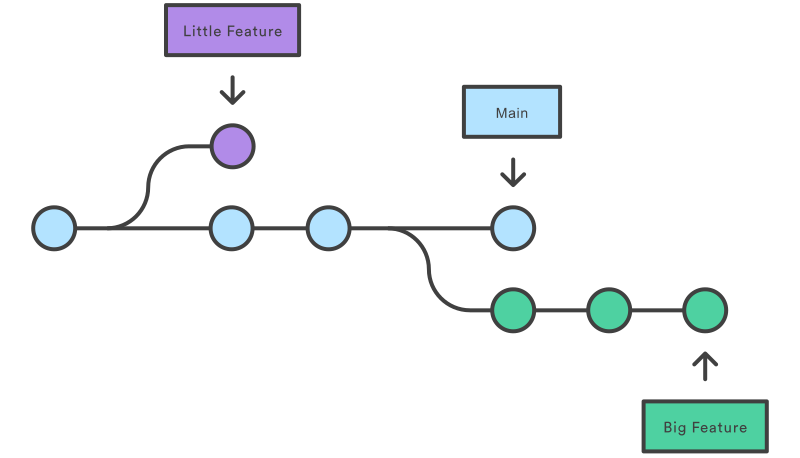
\includegraphics[width=0.88\textwidth]{Branches}
                  \end{onlyenv}
            \item<2-> They enable parallel development
                  \begin{itemize}
                      \item Implement new features
                      \item Fix bugs
                      \item Try out something
                      \item {}[\ldots]
                  \end{itemize}
            \item<2-> The always existing \;\PB{\texttt{main}}\; branch:
                  \begin{itemize}
                      \item By default created at initialization
                      \item Development should be done on other branches
                      \item Till few years ago it was called \;\PB{\texttt{master}}
                  \end{itemize}
        \end{itemize}
    \end{overlayarea}
\end{frame}
%~~~~~~~~~~~~~~~~~~~~~~~~~~~~~~~~~~~~~~~~~~~~%
\begin{frame}[fragile]{Git branch}
    \begin{lstlisting}[style=MyBash]
        # List all existing local branches
        $ git branch
        * @|\color{strings-color}main|@
    \end{lstlisting}
    \begin{lstlisting}[style=MyBash]
        # Create a new branch
        $ git branch new-branch
        $ git branch
        * @|\color{strings-color}main|@
        |+  new-branch+|
    \end{lstlisting}
    \begin{lstlisting}[style=MyBash]
        # Delete a branch
        $ git branch -d new-branch
        |+Deleted branch new-branch (was a45b032).+|
        $ git branch
        * @|\color{strings-color}main|@
    \end{lstlisting}
    \begin{varblock}{alert}[\textwidth]{Git is safe}
        \small
        If a modifications would be lost, Git does not allow you to delete the branch using the \texttt{-d} option.
        Use the \texttt{-D} option instead.
    \end{varblock}
\end{frame}
%~~~~~~~~~~~~~~~~~~~~~~~~~~~~~~~~~~~~~~~~~~~~%
\begin{frame}[fragile]{Git switch}
    \vspace{-8mm}
    \begin{overlayarea}{\textwidth}{0.8\textheight}
        \begin{varblock}{}[0.7\textwidth]{}
            \PB{This will in general change your workspace!}
        \end{varblock}
        \begin{lstlisting}[style=MyBash]
            # Switching to another branch
            $ git branch
            * @|\color{strings-color}main|@
            |+  new-branch+|
            $ git switch new-branch
            |+Switched to branch 'new-branch'+|
            $ git branch
            |+  main+|
            * @|\color{strings-color}new-branch|@
        \end{lstlisting}
        \begin{varblock}{alert}[\textwidth]{Git is safe}<only@1>
            \small
            You may switch branches with uncommitted changes in the work-tree if and only if said switching does not require clobbering those changes.
        \end{varblock}
        \begin{onlyenv}<2>
            \begin{lstlisting}[style=MyBash]
                # Creating and switching to a new branch at once
                $ git switch -c another-branch
                |+Switched to a new branch 'another-branch'+|
                $ git branch
                * @|\color{strings-color}another-branch|@
                |+  main+|
            \end{lstlisting}
        \end{onlyenv}
    \end{overlayarea}
\end{frame}
%~~~~~~~~~~~~~~~~~~~~~~~~~~~~~~~~~~~~~~~~~~~~%
\begin{frame}{Merging branches}
    \setlength{\leftmargini}{0.6cm}
    \begin{itemize}
        \item To merge means to unify the snapshots of two different branches
        \item This is automatically done by Git in a clever way
        \item When Git does not know how to merge the content of some file, it will create a conflict
        \item If conflicts occur, the merge will not automatically finish
        \item A merge can be aborted
        \item To fix conflicts, open and manually adjust files where Git failed
    \end{itemize}
    \medskip
    \begin{varblock}{alert}[0.65\textwidth]{}
        \alert{Git is safe, conflicts are not a bad thing!}
    \end{varblock}

\end{frame}
%~~~~~~~~~~~~~~~~~~~~~~~~~~~~~~~~~~~~~~~~~~~~%
\begin{frame}{Different types of merge}
%    \resizebox{1.1\textwidth}{!}{
    \hspace*{-3mm}
            \begin{tikzpicture}[node distance=4mm]
                \node (3W1) {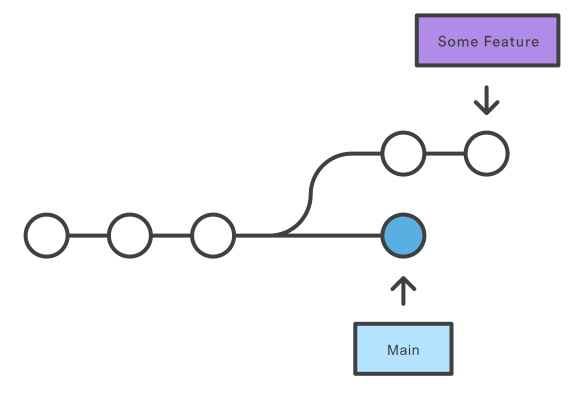
\includegraphics[width=0.42\textwidth]{Merge-3way_before}};
                \node[below = 1mm of 3W1.south west, anchor=north west] (3W2) {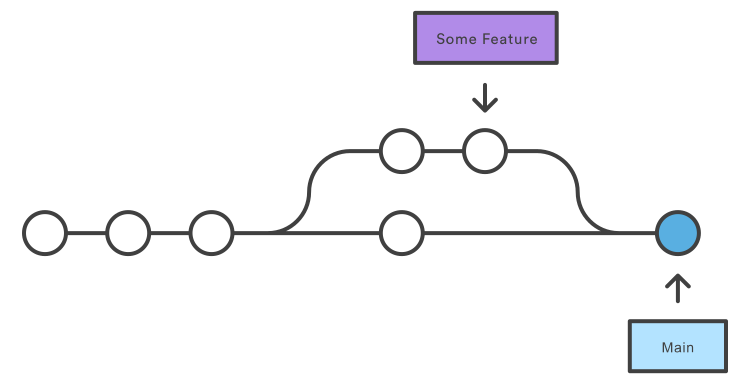
\includegraphics[width=0.52\textwidth]{Merge-3way_then}};
                \node[left  = of 3W1] (FF1) {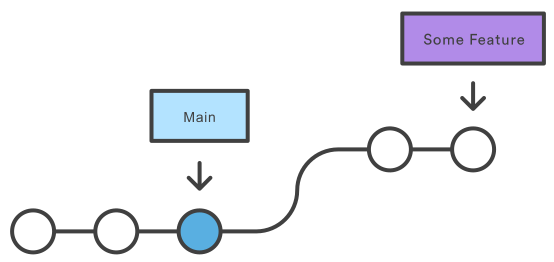
\includegraphics[width=0.38\textwidth]{Merge-FF_before}};
                \node[left  = of 3W2] (FF2) {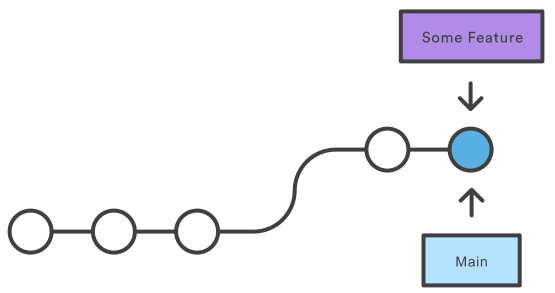
\includegraphics[width=0.38\textwidth]{Merge-FF_then}};
                \begin{scope}[every node/.style={font=\small}]
                    \node[left = 2mm of FF1] (BL) {\rotatebox{90}{Before}};
                    \node[left = 2mm of FF2] (AL) {\rotatebox{90}{After}};
                    \node[above = 34mm of 3W2] (3WL) {Three-way merge};
                    \node at (3WL -| FF1) (FFL) {Fast-forward merge};
                \end{scope}
                \draw ({$(FF1.east)!0.5!(3W1.west)$} |- FFL.north) -- ({$(FF1.east)!0.5!(3W1.west)$} |- 3W2.south);
                \draw ({$(FF1.south)!0.5!(FF2.north)$} -| AL.west) -- ({$(FF1.south)!0.5!(FF2.north)$} -| 3W2.east);
            \end{tikzpicture}
%        }
\end{frame}
%~~~~~~~~~~~~~~~~~~~~~~~~~~~~~~~~~~~~~~~~~~~~%
\begin{frame}[fragile]{Git merge: How does it work?}
    \setlength{\leftmargini}{5mm}
    \begin{enumerate}
        \item If possible, Git performs a fast-forward merge
        \item Otherwise a three-way merge is done and a new commit created
    \end{enumerate}
    \begin{varblock}{}[0.75\textwidth]{Be sure to be on the correct branch!}
        \begin{lstlisting}[style=MyBash, xrightmargin=11mm, xleftmargin=11mm, aboveskip=2mm]
            |+   +|git merge |+<source-branch>+|
        \end{lstlisting}
        It incorporates changes from the specified\\ branch into the present branch!
    \end{varblock}
    \vspace{3mm}
    \begin{lstlisting}[style=MyBash]
        # It is possible to force a three-way merge:
        $ git merge --no-ff |+<source-branch>+|
    \end{lstlisting}
\end{frame}
%~~~~~~~~~~~~~~~~~~~~~~~~~~~~~~~~~~~~~~~~~~~~%
\begin{frame}[fragile]{Merge conflicts: Fixing procedure}
    \begin{lstlisting}[style=MyBash, xleftmargin=-1mm, xrightmargin=-1mm]
        # A general example
        $ git merge <branch_name>
        |+Auto-merging <file>
        CONFLICT (content): Merge conflict in <file>
        Automatic merge failed; fix conflicts and then commit the result.+|
    \end{lstlisting}
    \begin{enumerate}
        \item Run \,\texttt{git status}\, to see \alert{unmerged paths}
        \item Find problematic hunks in files that contain conflicts\\
              \then Look for delimiters in the files:
%              {\footnotesize\ttfamily\begin{tabular}{c} <<<<<<<\\ =======\\ >>>>>>>\\ \end{tabular}}
              {~\footnotesize\texttt{<<<<<<<},\; \texttt{=======},\; \texttt{>>>>>>>}}
        \item Remove delimiters and adjust content
        \item Check the project works (e.g. compile, run tests)
        \item \texttt{git add}\, the files with fixed conflicts
        \item Commit added files\\
              \then Git propose you an auto-generated commit message
    \end{enumerate}
\end{frame}
%~~~~~~~~~~~~~~~~~~~~~~~~~~~~~~~~~~~~~~~~~~~~%
\AlertFrame{Live example!}
%===============================================================%


%===============================================================%
\section{Working with remote repositories}
%~~~~~~~~~~~~~~~~~~~~~~~~~~~~~~~~~~~~~~~~~~~~%
%git clone
%git fetch
%git pull
%git push
%===============================================================%


%===============================================================%
\section{A bare repository}
%~~~~~~~~~~~~~~~~~~~~~~~~~~~~~~~~~~~~~~~~~~~~%
%===============================================================%


%===============================================================%
\section{The stashing area}
%~~~~~~~~~~~~~~~~~~~~~~~~~~~~~~~~~~~~~~~~~~~~%
%===============================================================%


%===============================================================%
\section{The remaining git commands}
%~~~~~~~~~~~~~~~~~~~~~~~~~~~~~~~~~~~~~~~~~~~~%
%mv                Move or rename a file, a directory, or a symlink
%restore           Restore working tree files
%rm                Remove files from the working tree and from the index
%sparse-checkout   Initialize and modify the sparse-checkout
%
%bisect            Use binary search to find the commit that introduced a bug
%grep              Print lines matching a pattern
%
%rebase            Reapply commits on top of another base tip
%reset             Reset current HEAD to the specified state
%tag               Create, list, delete or verify a tag object signed with GPG
%===============================================================%



%~~~~~~~~~~~~~~~~~~~~~~~~~~~~~~~~~~~~~~~~~~~~%
\begin{frame}{That's \textbf{NOT} all folks}
    \vspace{0.02\textheight}
    \begin{enumerate}[<+->]
        \item Start using Git.
              \alert{\textbf{Now.}}
              Not tomorrow or next week, today!\\
              $\to\;$ Repeat what done on these slides
        \item Was anything unclear?
              Do you get stuck at some point?\\
              $\to\;$ Drop me \PP{\href{mailto:sciarra@itp.uni-frankfurt.de}{{\small\faEnvelope}\;an email}}
        \item Git is much more than this!\\
              $\to\;$ Come to next Z02 talk: \alert{\guillemotleft Let's git \textbf{together}\tikzmark{tg}\guillemotright}
    \end{enumerate}
    \begin{tikzpicture}[remember picture, overlay, scope on=<.->]
        \node[anchor=west, space=PT, text width=18mm] (content) at ($(tg)+(0.5,-0.8)$) {
            git clone\\
            git branch\\
            git switch\\
            git checkout\\
            git merge\\
            git pull\\
            git push
        };
        \path[to, shorter={0mm}{1mm}] ($(tg)-(0.6,0.25)$) edge[out=270, in=180] (content.west);
    \end{tikzpicture}
    \par\vspace{0.02\textheight}
    \begin{uncoverenv}<+->
        \begin{tikzpicture}[remember picture, overlay]
            \node[anchor=north east, cloud, aspect=3, cloud puffs=15, draw=PB, fill=PP!20, text=PB]
                at ($(current page.north east)+(-14mm,-6mm)$) {Thank you!};
        \end{tikzpicture}
        \begin{minipage}{0.8\textwidth}
            \begin{center}
                \large\bfseries\PQ{Believe me, it's worth it!}
            \end{center}
        \end{minipage}
    \end{uncoverenv}
\end{frame}
%===============================================================%

\end{document}
